\question
  Find all trees \(T\) such that \(\overline{T}\) is also a tree.

  \begin{solution}
    Recall that every tree of order \(n\) must have \(n-1\) edges. So, we want
    to find all trees such that \(|E(T)| = |E(\overline{T})|\). First, let us
    identify the possible orders of \(T\).
    \[
      \begin{aligned}
        n-1 &= \binom{n}{2} - (n-1) \\ 
        n-1 &= \frac{n(n-1)}{2} - (n-1) \\ 
        2(n-1) &= \frac{n(n-1)}{2} \\ 
        4n-4 &= n^2 - n \\ 
        0 &= n^2 - 5n + 4 \\ 
        0 &= (n-1)(n-4)
      \end{aligned}
    \]
    Hence, we have \(n=1, n=4\). For \(n=1\), we have that \(T=\overline{T}\)
    since it is just a single vertex and cannot be adjacent to anything.

    For \(n=4\), let us first identify all possible trees of order 4. 
    \begin{enumerate}
      \item One vertex connected to the rest. This does not work since
        \(\overline{T}\) would be disconnected. Namely, \(T\) has
        degree sequence \(\{3, 1, 1, 1\}\) but \(\overline{T}\)'s would be
        \(\{0, 2, 2, 2\}\)---meaning that one vertex has no neighbor.
        \begin{center}
          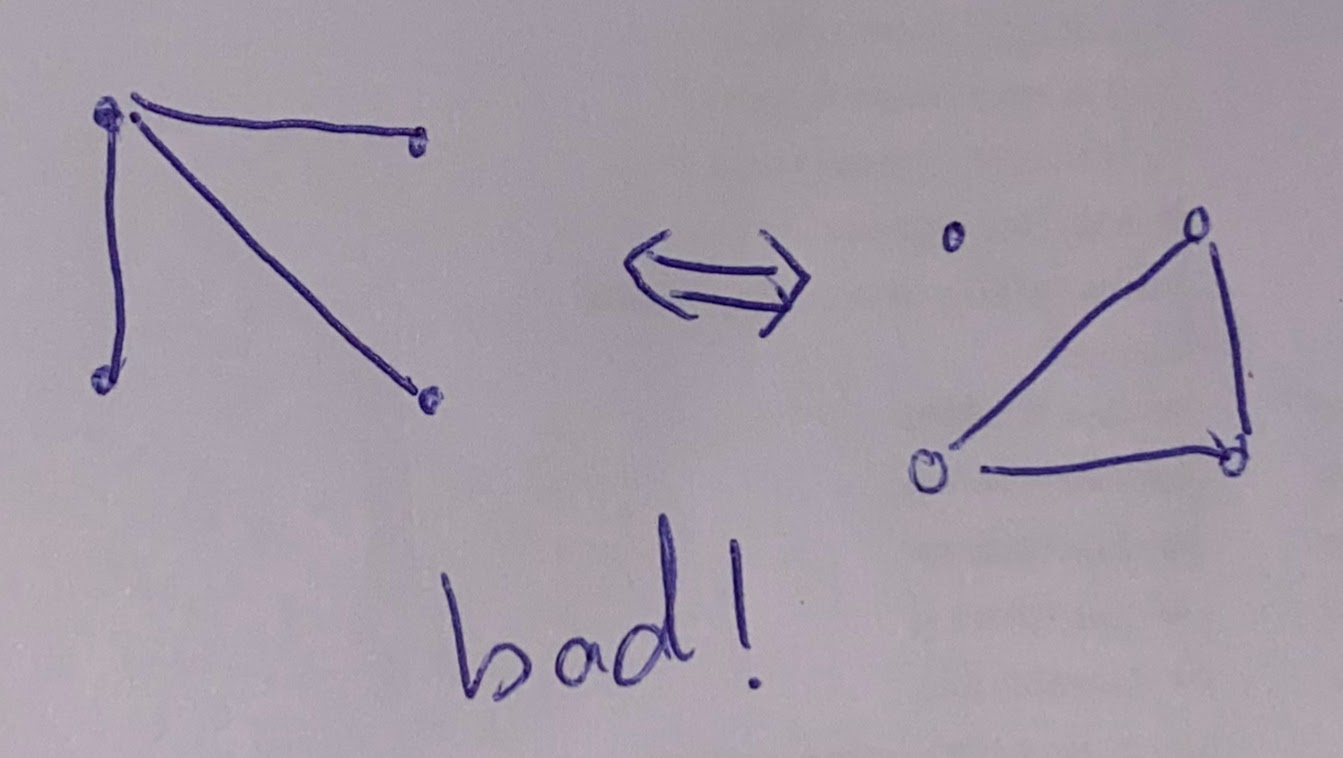
\includegraphics[width=0.31\textwidth]{figures/bad-p2}
        \end{center}
      \item Path of length 3 and graphs isomorphic to it. Notice that \(T\) has
        degree sequence \(\{1, 2, 2, 1\}\) and \(\overline{T}\) would have
        \(\{2, 1, 1, 2\}\) which is pretty much the same graph just slightly
        rotated/had vertices moved around.
        \begin{center}
          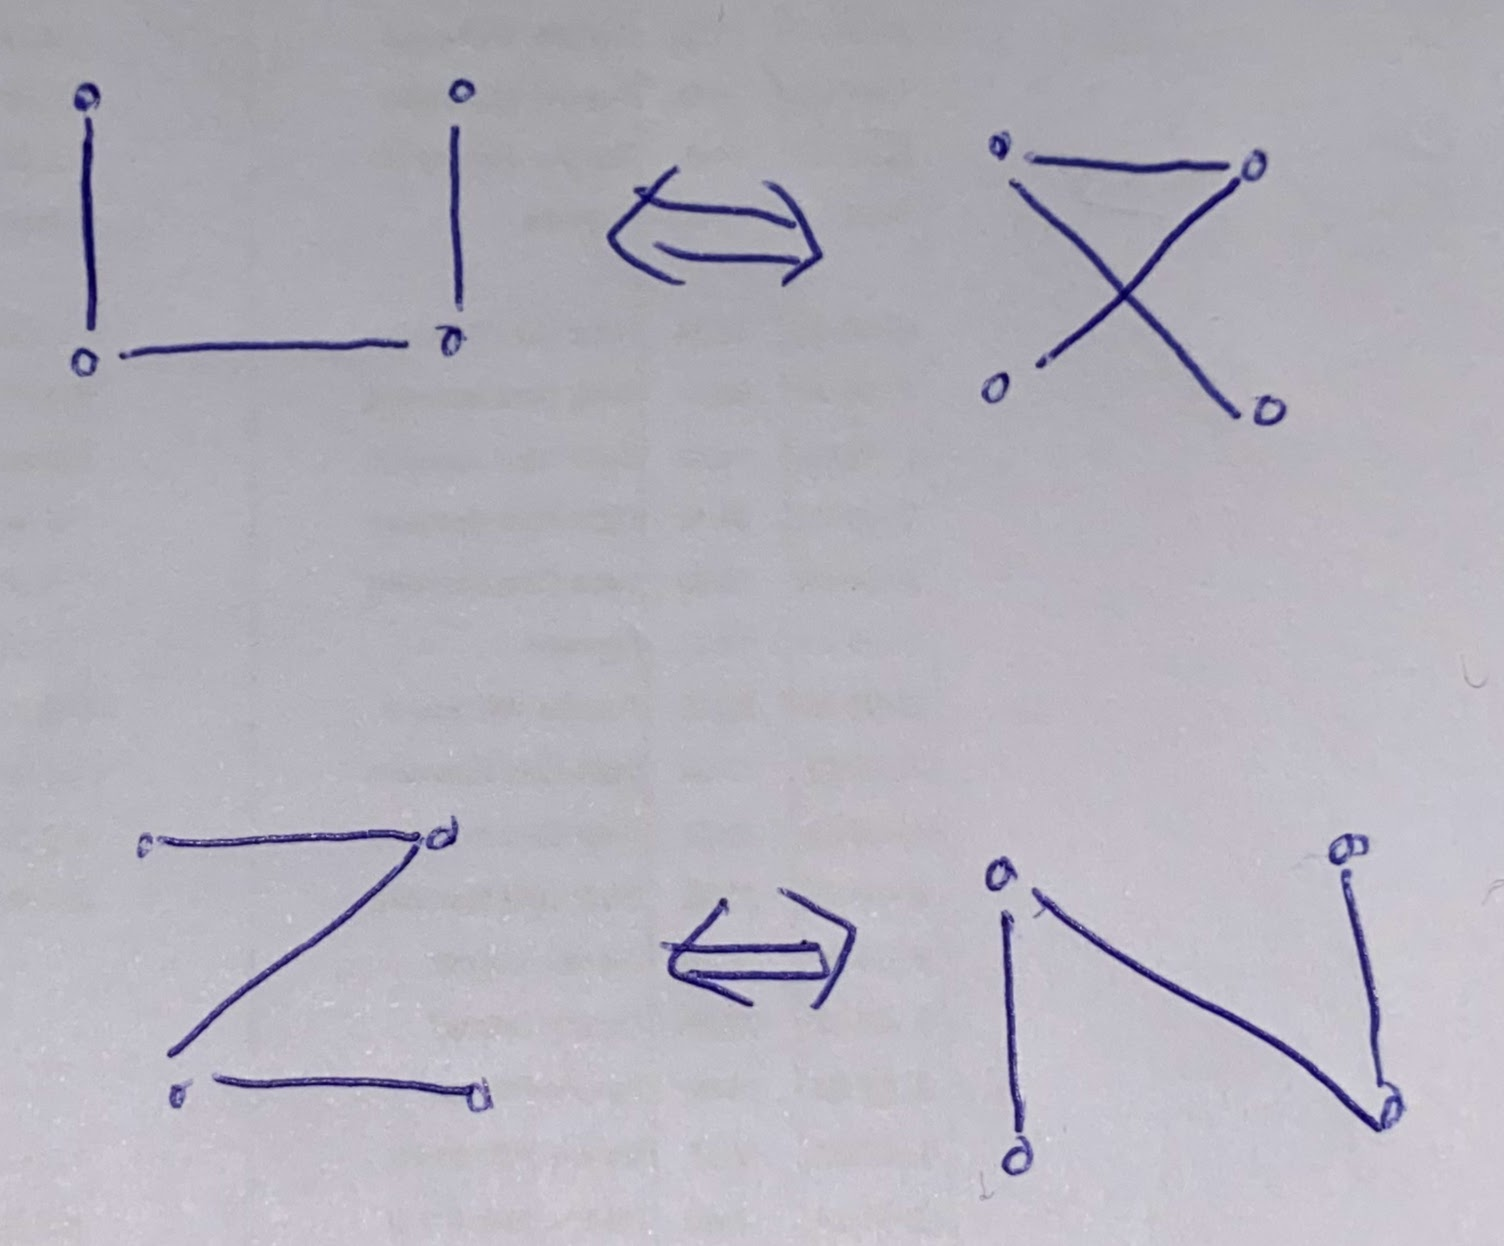
\includegraphics[width=0.31\textwidth]{figures/goodp2}
        \end{center}
    \end{enumerate}
    Note that we can verify that this is all by checking all non-isomorphic 
    graphs of order 4. Trust me Aj (diagram from \cite{sym13040710}).
    \begin{center}
      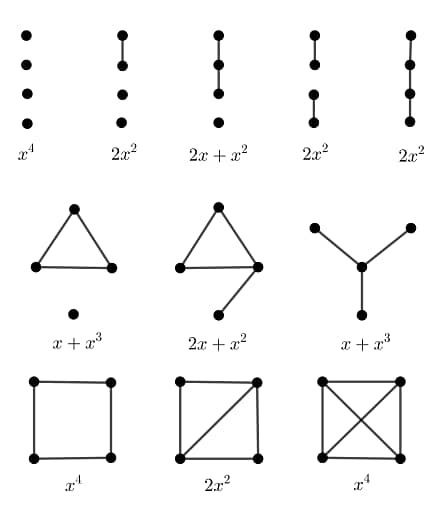
\includegraphics[width=0.4\textwidth]{figures/all4}
    \end{center}

    Therefore, we have that all trees \(T\) such that \(\overline{T}\) is also a
    tree are a tree of order 1 and a tree of order 4 where the tree is a path of
    length 3.
  \end{solution}
